\documentclass{article}

% if you need to pass options to natbib, use, e.g.:
% \PassOptionsToPackage{numbers, compress}{natbib}
% before loading nips_2016
%
% to avoid loading the natbib package, add option nonatbib:
% \usepackage[nonatbib]{nips_2016}

\usepackage[final]{nips_2016}

% to compile a camera-ready version, add the [final] option, e.g.:
% \usepackage[final]{nips_2016}

\usepackage[utf8]{inputenc} % allow utf-8 input
\usepackage[T1]{fontenc}    % use 8-bit T1 fonts
\usepackage{hyperref}       % hyperlinks
\usepackage{url}            % simple URL typesetting
\usepackage{booktabs}       % professional-quality tables
\usepackage{amsfonts}       % blackboard math symbols
\usepackage{nicefrac}       % compact symbols for 1/2, etc.
\usepackage{microtype}      % microtypography
\usepackage[pdftex]{graphicx}

\title{Deep learning in practice homework \protect\\ Self-driving cars in the DuckieTown environment \protect\\ DeepD(r)iveDucks team  \protect \\ Deep Learning a gyakorlatban házi feladat \protect\\ Önvezető autózás a DuckieTown környezetben \protect\\ DeepD(r)iveDucks csapat}

% The \author macro works with any number of authors. There are two
% commands used to separate the names and addresses of multiple
% authors: \And and \AND.
%
% Using \And between authors leaves it to LaTeX to determine where to
% break the lines. Using \AND forces a line break at that point. So,
% if LaTeX puts 3 of 4 authors names on the first line, and the last
% on the second line, try using \AND instead of \And before the third
% author name.

\author{
  Holló Áron\\
  MSc in Autonomous Vehicle Control Engineering\\
  Budapest University of Technology and Economics\\
  Budapest \\
  \texttt{holloaron7@gmail.com} \\
  \And
  Tóth Tibor Áron\\
  MSc in Autonomous Vehicle Control Engineering\\
  Budapest University of Technology and Economics\\
  Budapest \\
  \texttt{toth.tibor.aron@gmail.com} \\  
  \And
  Hajnal Bálint\\
  MSc in Mechatronics Engineering\\
  Budapest University of Technology and Economics\\
  Budapest \\
  \texttt{hajnal.balint.david@edu.bme.hu} \\  
}

\begin{document}
% \nipsfinalcopy is no longer used

\maketitle

\begin{abstract}

  Our team used the reinforcement learning based DAgger (Data Aggregation) algorithm implementation for the DuckieTown autonomous driving environment in order to complete the lane following challenge. In this challenge an affordable bot has to follow the lanes in a simplified route environment. The DAgger algorithm is imitation learning based, which means that it is a framework for learning a behavior policy from demonstrations. Being a reinforcement learning method, it uses rewards to approximate the best policy, which is the expert policy in the DAgger algorithm. It uses a teacher agent, the aformentioned expert, that shows the learner agent the correct decisions - when needed - based on the current image input data. We improved on the baseline algorithm by implementing custom hyperparameter tuning to find the best parameters for good results. The evaluation is executed in a simulation provided by Duckietown.
  
  Csapatunk a megerősített tanuláson alapuló Dagger (Adat Egyesítés) algoritmus implementációját használta a DuckieTown autonóm vezetési környezet sávkövetési kihívásának teljesítésére. A feladat egy robot mozgásának vezérlése úgy, hogy kövesse a sávokat egy utakkal ellátott egyszerűsített környezetben. A Dagger algoritmus az imitációs tanításon alapul, ami azt jelenti, hogy korábbi mintákra épülő viselkedési stratégia megtanulására szolgáló keretrendszer. Mivel ez egy megerősített tanulási módszer, ezért jutalmakkal erősítjük meg a helyes viselkedést, ami a “szakértő” viselkedése. Ez a szakértő a tanító ágens, ami szükség esetén megmutatja a helyes döntéseket a bemeneti képadatok alapján. Az alap algoritmust továbbfejlesztettük egyedi hiperparaméter optimalizációval, hogy megtaláljuk azokat a tanítási paramétereket, amikkel a legjobb eredményt érhetjük el tanítás során. A kiértékelés a DuckieTown platform szimulációján keresztül történik. 
  
\end{abstract}

\section{Introduction}

The DuckieTown platform is both a physical and virtual environment, where people can study machine learning and artificial intelligence for self-driving cars. The platform has a competition, where students from all over the world can compete on who can make the most successful DuckieBot. Competitors often train their machine learning models in a virtual environment, which has an equal looking physical counterpart where the models can be seen working in real life. The virtual environment provides a cheap and easily accessible way to conduct machine learning research. Due to every solution being based on computer vision, the results from the virtual environments carry over to the real world pretty consistently. \\


\section{Topic description}

There are several implementation methods for the DuckieTown challenges due to the fact that computer vision is a very wide topic, and also there are several challenge types. We wanted to create an implementation for the lane keeping challenge, where the goal is to keep the so-called DuckieBot on the track in the randomly generated environment and achieve the furthest distance in a given time.

We chose an imitation learning algorithm called "DAgger", that is "Data Aggregation" for our implementation. Imitation learning is a reinforcement learning method, which uses an expert solution to reward the agent. In a self-driving car environment it is really hard to manually design a reward function, and the imitation learning solves this problem. The expert provides a set of demonstration to the agent to learn from. The agent tries to learn, mimic the optimal policy by imitating the expert's solution. The problem with a simple imitation learning algorithm is that the training data is not identically and evenly distributed, which means that if the agent is not following the expert's trajectory properly, and deviates from it, then it can reach a state from where it can not recover to the optimal track, because the expert never experienced that state. Robustness is not guaranteed in this solution. This is what the "DAgger" or Data Aggregation algorithm offers a solution for. The agent interacts with the environment, but sometimes the expert takes over control to help recovery. They are changed randomly hoping that the expert will help in recovering, therefore learning takes place. 

Due to the Data Aggregation algorithm baseline being available to us, our main goal was to study the system and improve it. We executed custom hyperparameter optimisation on an existing implementation of the algorithm.

\subsection{Previous solutions}

The challenges are solved with a wide range of approaches. Our focus was mainly on "DAgger" algorithm solutions.

The "DAgger" algorithm was initially developed by Stephane Ross and his co-authors in 2011 \citep {ross2011reduction}.The baseline "DAgger" solution provided for the competitors on the official website - which we tried to improve - is based on the paper by Diaz and Manfred \citep{diaz2018interactive}, the previusly mentioned original algorithm \citep {ross2011reduction} and a solution made for drones to drive on the streets \citep {loquercio2018dronet}. They developed an example of a system which aims to help visually impaired people cross intersections by capturing the knowledge of sighted people. They also developed a theoretical and experimental framework for consistent performance in different environments. More research around DAgger algorithm can be read in these papers: \citep{prakash2020exploring} \citep{bicer2019sample} \citep{cui2019uncertainty} \citep{kamrani2020mariodagger} \citep{elers2019continual} \citep{hussein2017imitation} \citep{DBLP:journals/corr/abs-1901-04772}.



\section{System plan}

Due to using an existing solution, we first needed to study its system in order to improve it. The program is written in Python, and it uses the PyTorch machine learning framework. 

\verb|train.py| is the script, that starts the training based on the arguments passed in. We implemented our hyperparameter optimisation in \verb|train_tune.py|, which is based on this script. 

The \verb|dronet.py| file contains the architecture of the neural network based on Dronet \citep{loquercio2018dronet}. Its a convolutional network consisting of a 5x5 convolutional filter, a 3x3 max pooling layer, 3x3 convolutional filters, a dropout filter and ReLU activation. The outputs are the steering angle and acceleration. 

\verb|pure_pursuit_policy.py| contains the teacher algorithm, which projects a point for the agent to follow. 

\verb|test.py| is used to test a model, after passing it in to the script. 

\verb|dataset.py| optimizes RAM usage by storing arrays on disk. 

\verb|neural_network_policy.py| is a wrapper to train a neural network model. It takes a pytorch mode, and an optimiser as inputs among others, and uses the expert actions to predict. 

\verb|dagger.py| is the "DAgger" algorithm, which is used to mix policies between learner and expert. 

\verb|iil_learning.py| contains the main imitation learning algorithm. 

\section{Implementation}

\subsection{Data acquisiton, preparation}

The teaching is done by an expert agents actions this is how the data is acquired for learning. The agent can either be controlled by a human in the virtual simulator, or by a preprogrammed algorithm. The data received by the learner are the images in 120x160 size from the DuckieBots' vision, and the expert actions. 

\subsection{Teaching}

The learner agent tries to follow the teacher, and predict the correct actions. If the learner starts to deviate from the track too much, then the control is given back to the expert. It is controlled by thresholds. The convergence angle threshold is for the angle deviation between the expert and the learner. The convergence distance threshold is for the distance between the learner and expert's trajectory.

\subsection{Evaluation}


We calculated the average loss after each episode to compare them. The loss function takes into consideration the velocity and the steering angle of the learning agent and the expert. For the velocity, the binary cross entropy loss is used with a sigmoid function. A decay factor is also used to for the velocity loss.  For the steering angle the mean squared error is calculated. The cumulated error is their added loss.

We implemented a grid search hyperparameter optimization for the teaching. The parameters space we considered to iterate through was: 
\begin{itemize}

\item episode number: 10, 15
\item horizon: 64, 128, 256
\item learning rate: 1e-1, 1e-2, 1e-3, 1e-4
\item learning rate decay: 0.5, 0.6, 0.7, 0.8
\item batch size: 16, 32.
\newpage

\end{itemize}

\begin{figure}
    \centering
    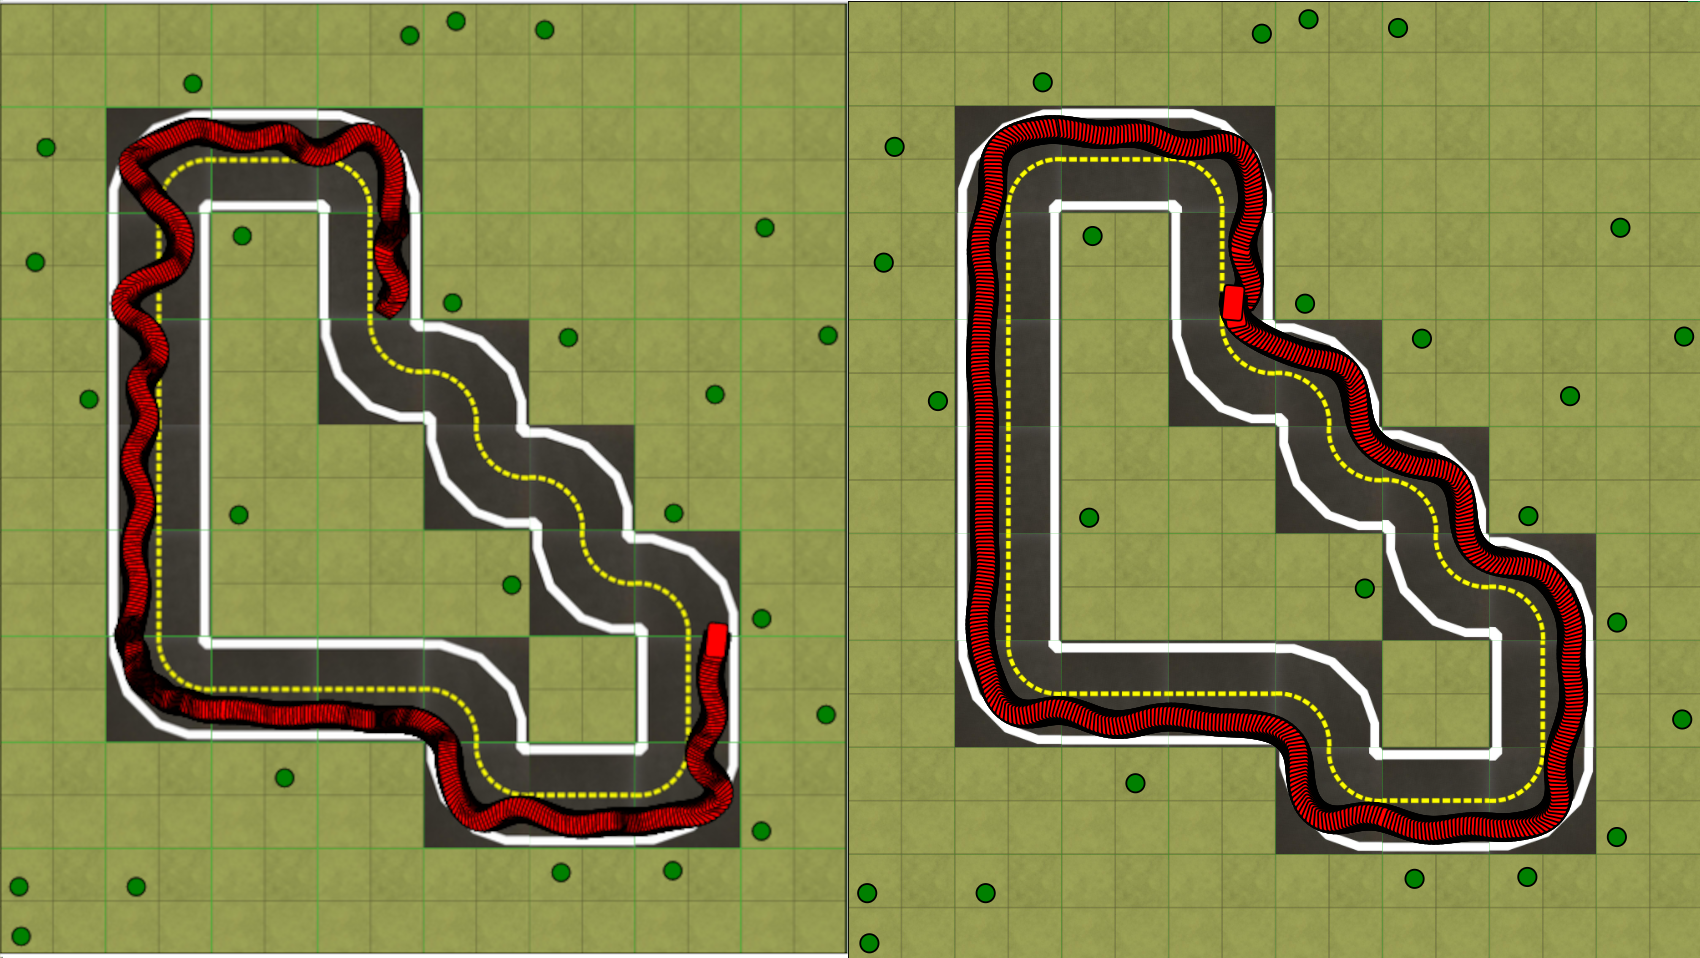
\includegraphics[width=0.8\linewidth]{eredmeny_egyben.png}
    \caption{The best result from the baseline solution (left) and the hyperparameter optimisation (right)}
    \label{fig:result}
\end{figure}


\begin{table}[t]
  \caption{Comparing Duckietown metrics for each solution}
  \label{sample-table}
  \centering
  \begin{tabular}{lll}
   \toprule
    Metrics     & Baseline     & Hyperparameter optimised \\
    \midrule
    Driving distance [m] &  10,1  & 12,5     \\
    Survival time [s] &  60  &  60    \\
    Heading deviation [$^{\circ}$] & 15.14 & 10.46 \\
    \bottomrule
  \end{tabular}
\end{table}

The best results of the DAgger baseline solution and our hyperparameter optimized solution for this map can be seen on figure 1. Both of the solution were able to stay on the track during the run, but as it can be seen in table 1, the running distance - which is the main deciding factor - differs. We were able to run the duckie bot around 1/5th further on the track. The heading deviation also outperformed the baseline, which means the robot was able to run much more smoothly, with less waddling.

\subsection{Testing}

Due to the fact that we are not working with existing data, but rather "live" data created on the fly, our solution didn't use testing.\\ 


\section{Conclusion, future plans}

We spent a lot of time figuring out how the baseline works, where can we make modifications to implement what we wanted. Setting up the docker image and a cloud based computer with a jupyterlab for the training, testing, evaluating needed much more time for us than anticipated, because we are not really experienced with these systems. We set up Tensorboard for our hyperparameter and metric logging, so we could see the loss functions for each episode and the hyperparameter set of each models. Complications also occured from large files that the tensorboard produced during plotting, which filled up the memory of the cloud computer.
These things set us back on time unfortunately, therefore we didn't really had time to implement all our plans.


Despite being successful at the lane following task, there are always more ways for improvement. It would be beneficial to implement hyperparameter optimisation over a wider range of possible parameters to get more accurate results. Another improvement could be better teacher algorithm, or a different neural network architecture. 





% \section*{References} % (eredeti)

\medskip

\small

\bibliographystyle{plain}
\bibliography{references}


\end{document}
